\documentclass[a4paper]{article}
\addtolength{\hoffset}{-2.25cm}
\addtolength{\textwidth}{4.5cm}
\addtolength{\voffset}{-3.25cm}
\addtolength{\textheight}{5cm}
\setlength{\parindent}{15pt}

\usepackage[unicode=true, colorlinks=false, hidelinks]{hyperref}
\usepackage[utf8]{inputenc}
\usepackage[english, russian]{babel}
\usepackage{mathtext}
\usepackage[T2A, TS1]{fontenc}
\usepackage{microtype} % Slightly tweak font spacing for aesthetics
\usepackage{amsthm, amssymb, amsmath, amsfonts, nccmath}
\usepackage{nicefrac}
\usepackage{epstopdf}
\usepackage[export]{adjustbox}
\usepackage{float} % Improved interface for floating objects
\usepackage{graphicx, multicol} % Enhanced support for graphics
\usepackage{pdfrender,xcolor}
\usepackage{breqn}
\usepackage{mathtools}
\usepackage{titling}
\usepackage{bm}
\usepackage{centernot}
\usepackage[cal=boondoxo,calscaled=.96]{mathalpha}
\usepackage{marvosym, wasysym} % More symbols
\usepackage{rotating} % Rotation tools
\usepackage{censor} % Facilities for controlling restricted text
\usepackage{indentfirst}
\usepackage{svg}

\DeclareMathOperator{\rad}{rad}
\DeclareMathOperator{\imid}{mid}
\DeclareMathOperator{\sign}{sign}
\newcommand{\mbb}[1]{\mathbb{#1}}
\newcommand{\mbf}[1]{\mathbf{#1}}

\usepackage{array}
\newcolumntype{C}[1]{>{\centering\let\newline\\\arraybackslash\hspace{0pt}}m{#1}}

\usepackage{fancyhdr}
\pagestyle{fancy}
\fancyhead{}\renewcommand{\headrulewidth}{0pt}
\fancyfoot[L]{}
\fancyhead{}
\fancyfoot{}
\fancyfoot[R]{\thepage}
\begin{document}
\large
\begin{center}
    Санкт-Петербургский политехнический университет\\
    Высшая школа прикладной математики и\\вычислительной физики,\\ 
    Физико-механический институт\\
    \vspace{3em}
    Направление подготовки\\
    01.03.02 «Прикладная математика и информатика»\\
    \vspace{10em}
    \Large
    Отчет по курсовому проекту \\
    по дисциплине «Интервальный анализ»\\
    на тему «Интервальная регрессия несовместных групп данных»
    \vspace{17em}
    \large
\end{center}
Выполнил студент гр. 5030102/80201\\
Кирпиченко С. Р.\\
Руководитель\\
Баженов А. Н.
\vspace{10.5em}
\begin{center}
    Санкт-Петербург\\
    2022
\end{center}
\thispagestyle{empty}
\newpage
\tableofcontents
\addtocontents{toc}{~\hfill\textbf{Страница}\par}
\newpage
\listoffigures
\addtocontents{lof}{~\hfill\textbf{Страница}\par}
\newpage
\listoftables
\addtocontents{lot}{~\hfill\textbf{Страница}\par}
\newpage
\section{Постановка задачи}
Для предоставленных данных 
\begin{table}[H]
    \centering
    \begin{tabular}{|c|c|}
        \hline
         $x$&$y$  \\
         \hline
         0&30\\
         \hline
         64&30\\
         \hline
         128&26\\
         \hline
         192&24\\
         \hline
         256&17\\
         \hline
         320&11\\
         \hline
         384&7\\
         \hline
         448&0\\
         \hline
         384&6\\
         \hline
         320&7\\
         \hline
         256&11\\
         \hline
         192&14\\
         \hline
         128&20\\
         \hline
         64&25\\
         \hline
         0&29\\
         \hline
    \end{tabular}
    \caption{Исходные данные}
    \label{tab:data}
\end{table}
Рассматривается задача построения интервальной регрессии $\mbf{X}\beta=\mbf{y}$. Необходимо провести линейный регрессионный анализ и добиться совместности выборки посредством введения в рассмотрение интервальных величин. Необходимо провести вычисления и привести иллюстрации:
\begin{itemize}
    \item Обработки данных посредством введения интервальных величин в отклик
    \item Обработки данных посредством введения брусов совместности, добиться сильной линейной совместности интервальных данных
    \item Обработки данных как единого целого с помощью метода квадратных подсистем
\end{itemize}
\section{Теория}
\subsection{Понятие накрывающей и совместной выборки}
Брус неопределенности измерения называется накрывающим, если он гарантированно содержит истинные значения измеряемых величин входных и выходных переменных зависимости. Иначе брус называется ненакрывающим.

Накрывающей выборкой называется совокупность накрывающих измерений. Если в выборке содержится хотя бы одно ненакрывающее измерение, то в таком случае она называется ненакрывающей. 

Данное определение тесно связано с понятием совместности. Если имеются точные измерения предикторных переменных и некоторые неопределенности в измерении отклика, то в таком случае построенная нами линейная регрессия называется совместной (согласованной) с данными, если ее график проходит через все отрезки неопределенности. 
\subsection{Слабая и сильная совместность}
Функциональная зависимость называется слабо совместной с данными, если ее график проходит через каждый брус неопределенности измерений хотя бы для одного значения аргумента. 

Функциональная зависимость называется сильно совместной с данными, если ее график проходит через каждый брус неопределенности измерений для любого значения аргумента из интервалов неопределенности входных переменных.
\subsection{Алгоритм достижения совместности входных данных}
Для решения поставленной задачи будет использован аппарат линейного программирования. Каждая точка исходных данных будет интерпретирована как середина отрезка неопределенности, который будет расширяться для достижения совместности выборки. В ходе решения составленной задачи линейного программирования будут получены коэффициенты регрессии $\beta$ и величины $\rad{\mbf{y}_i}=w_i$, минимизированные по норме из пространства $\mathcal{l}_1$. 

Формальная постановка задачи:
\begin{equation}\label{alg1}
\begin{cases}
        x_i\beta_1+\beta_0\leq y_i + w_i,& i=\overline{1,n}\\
        x_i\beta_1+\beta_0\geq y_i - w_i,& i=\overline{1,n}\\
        f(\beta,w)=\sum w_i\rightarrow \min        
\end{cases}
\end{equation}
В результате решения симплекс методом находятся $n+2$ параметра.
\subsection{Алгоритм достижения сильной совместности интервальных брусов}
Идейно аналогичен предыдущему алгоритму, вводятся дополнительные величины для расширения неопределенности входных данных по координате предиктора. Для сохранения линейности постановки необходимо задавать коэффициент наклона прямой $\beta_1$ извне. Минимизируется сумма коэффициентов расширения брусьев. 

Формальная постановка задачи:
\begin{equation}\label{alg2}
\begin{cases}
        (x_i-q_i)\beta_1+\beta_0\leq y_i + w_i,& i=\overline{1,n}\\
        (x_i+q_i)\beta_1+\beta_0\geq y_i - w_i,& i=\overline{1,n}\\
        f(\beta_0,q,w)=\sum w_i+\sum q_i\rightarrow \min
\end{cases}
\end{equation}
Постановка знаков после величин $x_i$ обусловлена отрицательной корреляцией исходных данных. Итого в результате решения задачи получается $2n+1$ параметр.
\subsection{Алгоритм обработки данных в целом}
Для использования данного метода необходимо перейти из $\mbb{IR}$ в полную интервальную арифметику $\mbb{KR}$. Две несовместные «ветви» исходных данных ($\mbf{y}_k^1$ и $\mbf{y}_k^2$) рассматриваются вместе.

Алгоритм:
\begin{enumerate}
    \item Составляем вектор минимумов по включению $\mbf{y}_k=\mbf{y}_k^1\bigwedge\mbf{y}_k^2=[\max\{\underline{\mbf{y}}_k^1,\underline{\mbf{y}}_k^2\}, \min\{\overline{\mbf{y}}_k^1,\overline{\mbf{y}}_k^2\}]$
    \item Решаем задачу нахождения максимума совместности: $\mbf{X}\beta\subseteq\mbf{y}$
    \item Получив переопределенную ИСЛАУ, воспользуемся методом квадратных подсистем. Исходная ИСЛАУ разбивается на несколько более мелких $\mbf{X}^{(1)}\beta=\mbf{y}^{(1)},\dots,\mbf{X}^{(m)}\beta=\mbf{y}^{(m)}$ c квадратными матрицами $\mbf{X}^{(i)}$. 
    \item Данные системы решаются известными численными методами (в данной работе - субдифференциальным методом Ньютона), после чего строится пересечение полученных оценок множеств решений $\Xi=\bigcap_{i=1}^m\Xi_i$.
    \item Множество $\Xi$ является оценкой информационного множества для исходных несовместных данных.
\end{enumerate}
\section{Реализация}
Для осуществления вычислений и визуализации результатов использовалась среда Octave с пакетом интервальной арифметики interval и сторонней библиотекой полной интервальной арифметики kinterval. Для решения задач линейного программирования использовалась функция glpk.
\section{Результаты}
Как было описано выше, исходные данные отрицательно коррелированы. Можно выделить две квазилинейных «ветви», изображенных синим и красным цветом на графике ниже.
\begin{figure}[H]
    \centering
    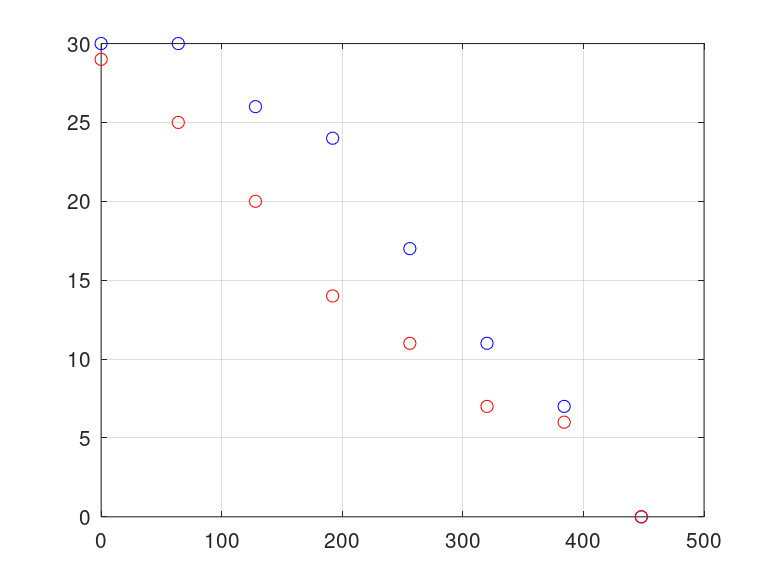
\includegraphics[width=15cm]{img/data.png}
    \caption{Исходные точечные данные}
    \label{fig:data}
\end{figure}
\subsection{Обработка данных посредством введения интервальных величин в отклик}
Рассмотрим выделенные выше ветви данных по отдельности и воспользуемся алгоритмом \ref{alg1}. Результаты приведены на графике ниже. Цветовые обозначения ветвей сохранены.
\begin{figure}[H]
    \centering
    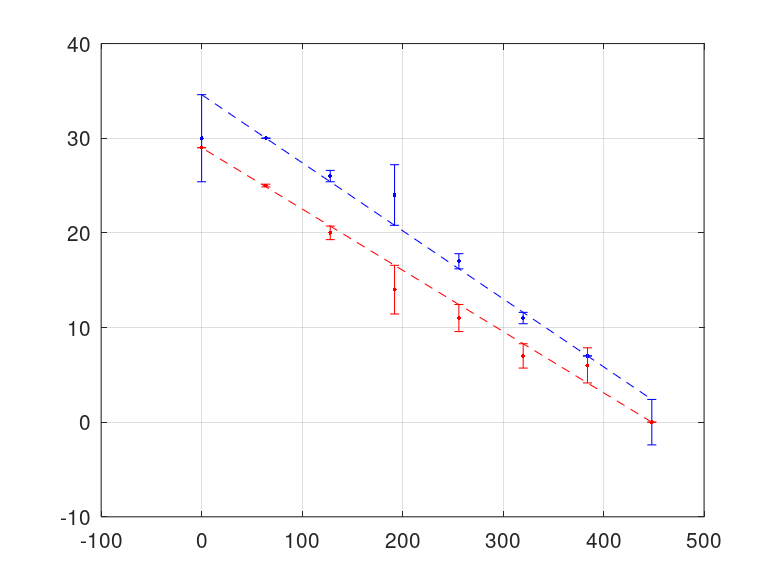
\includegraphics[width=13cm]{img/branches.png}
    \caption{Достижение совместности данных для разных ветвей}
    \label{fig:branches}
\end{figure}
Для синей ветви данных получены следующие результаты: $\beta_0=34.6,\:\beta_1\approx-0.072,\:||w||_1=12.2$. Для красной ветви: $\beta_0=29,\:\beta_1\approx-0.065,\:||w||_1\approx8$.

Обработаем всю выборку и добьемся ее совместности.
\begin{figure}[H]
    \centering
    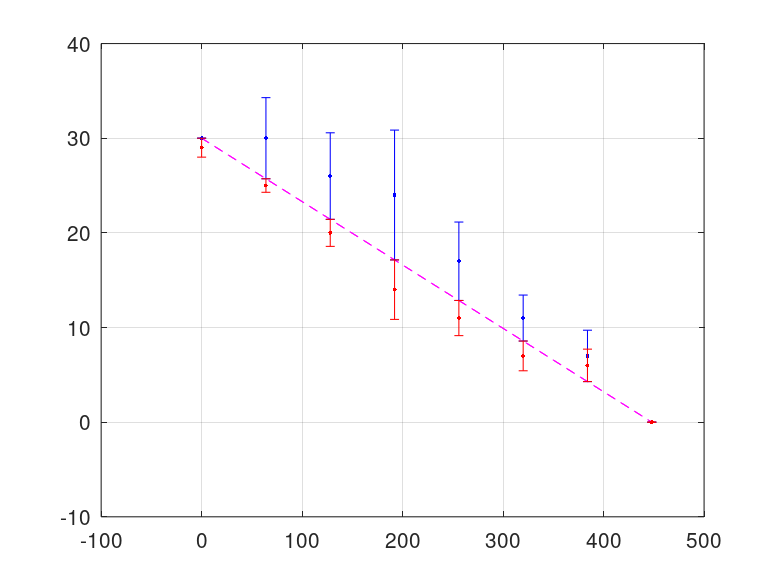
\includegraphics[width=13cm]{img/res_1.png}
    \caption{Достижение совместности данных для всей выборки}
    \label{fig:res_1}
\end{figure}
Численные результаты: $\beta_0=30,\:\beta_1\approx-0.067,\:||w||_1\approx36.43$.
\subsection{Обработка данных посредством введения брусов совместности}
Алгоритму \ref{alg2} нет смысла искусственно расширять брусы по координате предиктора, так как в случае точечной матрицы $X$ совместная выборка (например, полученная в предыдущем пункте) сильно совместна по определению. Ввиду этого введем неопределенность в координату $x$ каждой исходной точки так, что $\rad\mbf{x}_i=\frac{1}{4}(x_2-x_1)=16$. Координаты брусов $\mbf{y}$ получены следующим образом: $\mbf{y}_k=[\min\{y_k^1,y_k^2\}, \max\{y_k^1,y_k^2\}]$. Коэффициент $\beta_1$ возьмем из результатов построения регрессии в предыдущем пункте, $\beta_1\approx-0.067$.
\begin{figure}[H]
    \centering
    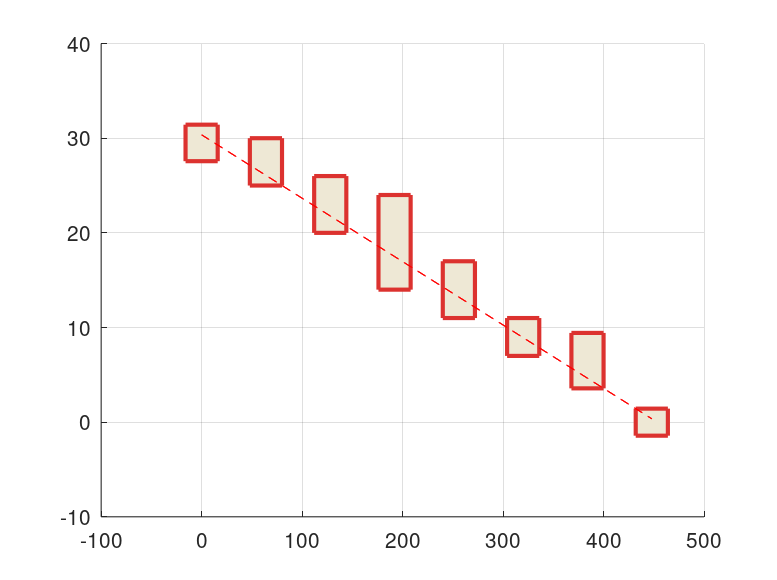
\includegraphics[width=15cm]{img/res_2.png}
    \caption{Сильная линейная совместность для интервальных предиктора и отклика}
    \label{fig:res_2}
\end{figure}
Численные результаты: $\beta_0\approx30.36,\:||w||_1\approx5.29,\:||q||_1=0$.
\subsection{Обработка данных как единого целого с помощью метода квадратных подсистем}
Для построения регрессии данным методом в данные была добавлена неопределенность: $\rad\mbf{x}_i=16,\:\rad\mbf{y}_i=1$. Результат операции взятия минимумов по включению:
\begin{table}[H]
    \centering
    \begin{tabular}{|c|c|}
        \hline
         $x$&$y$  \\
         \hline
         [-16,16]&[29,30]\\
         \hline
         [48,80]&[29,26]\\
         \hline
         [112,144]&[25,21]\\
         \hline
         [176,208]&[23,15]\\
         \hline
         [240,272]&[16,12]\\
         \hline
         [304,336]&[10,8]\\
         \hline
         [368,400]&[6,7]\\
         \hline
         [432,464]&[-1,1]\\
         \hline
    \end{tabular}
    \caption{$\mbf{y}_k^1\bigwedge\mbf{y}_k^2$}
    \label{tab:kint}
\end{table}
Для решения переопределенной системы она была разбита на 6 частей: ИСЛАУ $2\times2$, каждая смещена на строку ниже относительно предыдущей. Решение получено с помощью субдифференциального метода Ньютона из библиотеки kinterval. 

Таблица результатов решения ИСЛАУ методом квадратных подсистем:
\begin{table}[H]
    \centering
\begin{tabular}{|c|c|}
    \hline
     Номера строк исходной ИСЛАУ& $\Xi_i$ \\
     \hline
     $1,2$&$\begin{pmatrix}[0,-0.083333] \\ [29,30]\end{pmatrix}$\\
     \hline
     $2,3$&$\begin{pmatrix}[-0.0625,-0.078125] \\ [34,29.75]\end{pmatrix}$\\
     \hline
     $3,4$&$\begin{pmatrix}[-0.03125,-0.09375] \\ [29.5,31.5]\end{pmatrix}$\\
     \hline
     $4,5$&$\begin{pmatrix}[-0.10938,-0.046875] \\ [45.75,23.25]\end{pmatrix}$\\
     \hline
     $5,6$&$\begin{pmatrix}[-0.09375,-0.0625] \\ [41.5,27]\end{pmatrix}$\\
     \hline
     $6,7$&$\begin{pmatrix}[-0.0625,-0.015625] \\ [31,12.75]\end{pmatrix}$\\
     \hline
\end{tabular}
\caption{Результаты метода квадратных подсистем}
\label{tab:xi}
\end{table}
Пересечение $\Xi=\bigcap_{i=1}^m\Xi_i$ обозначено на следующем графике красным цветом.
\begin{figure}[H]
    \centering
    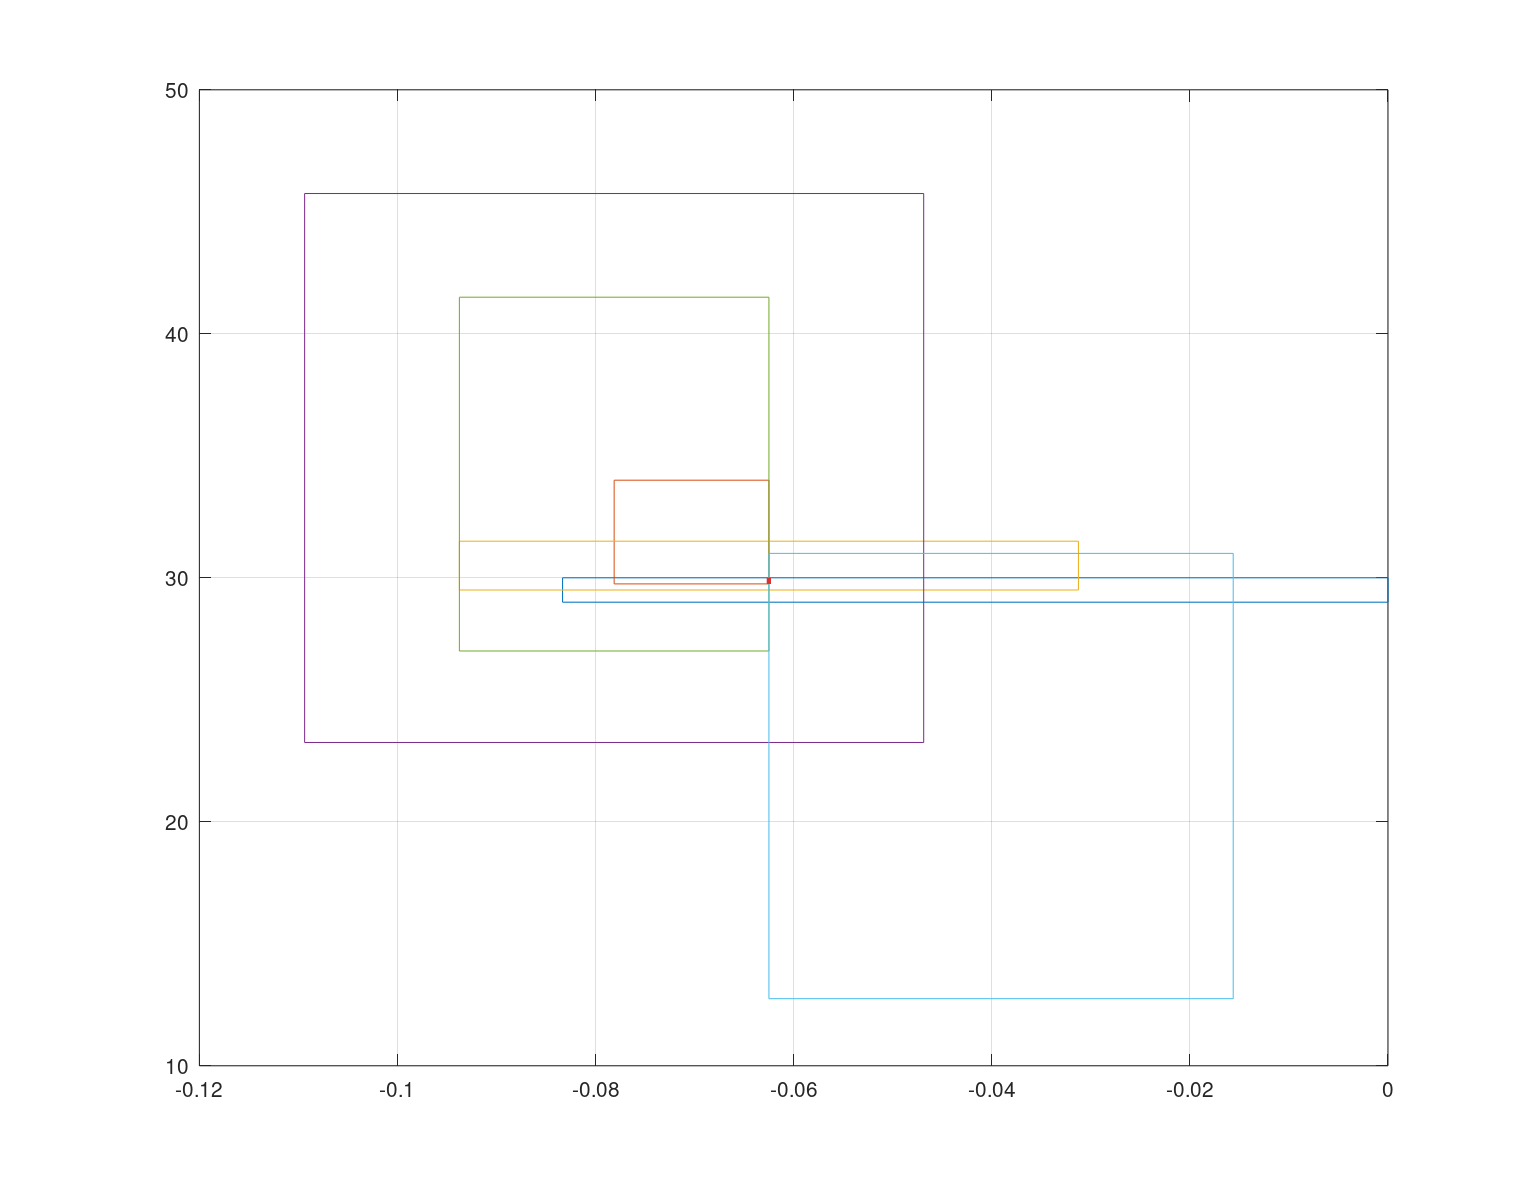
\includegraphics[width=8cm]{img/boxes.png}
    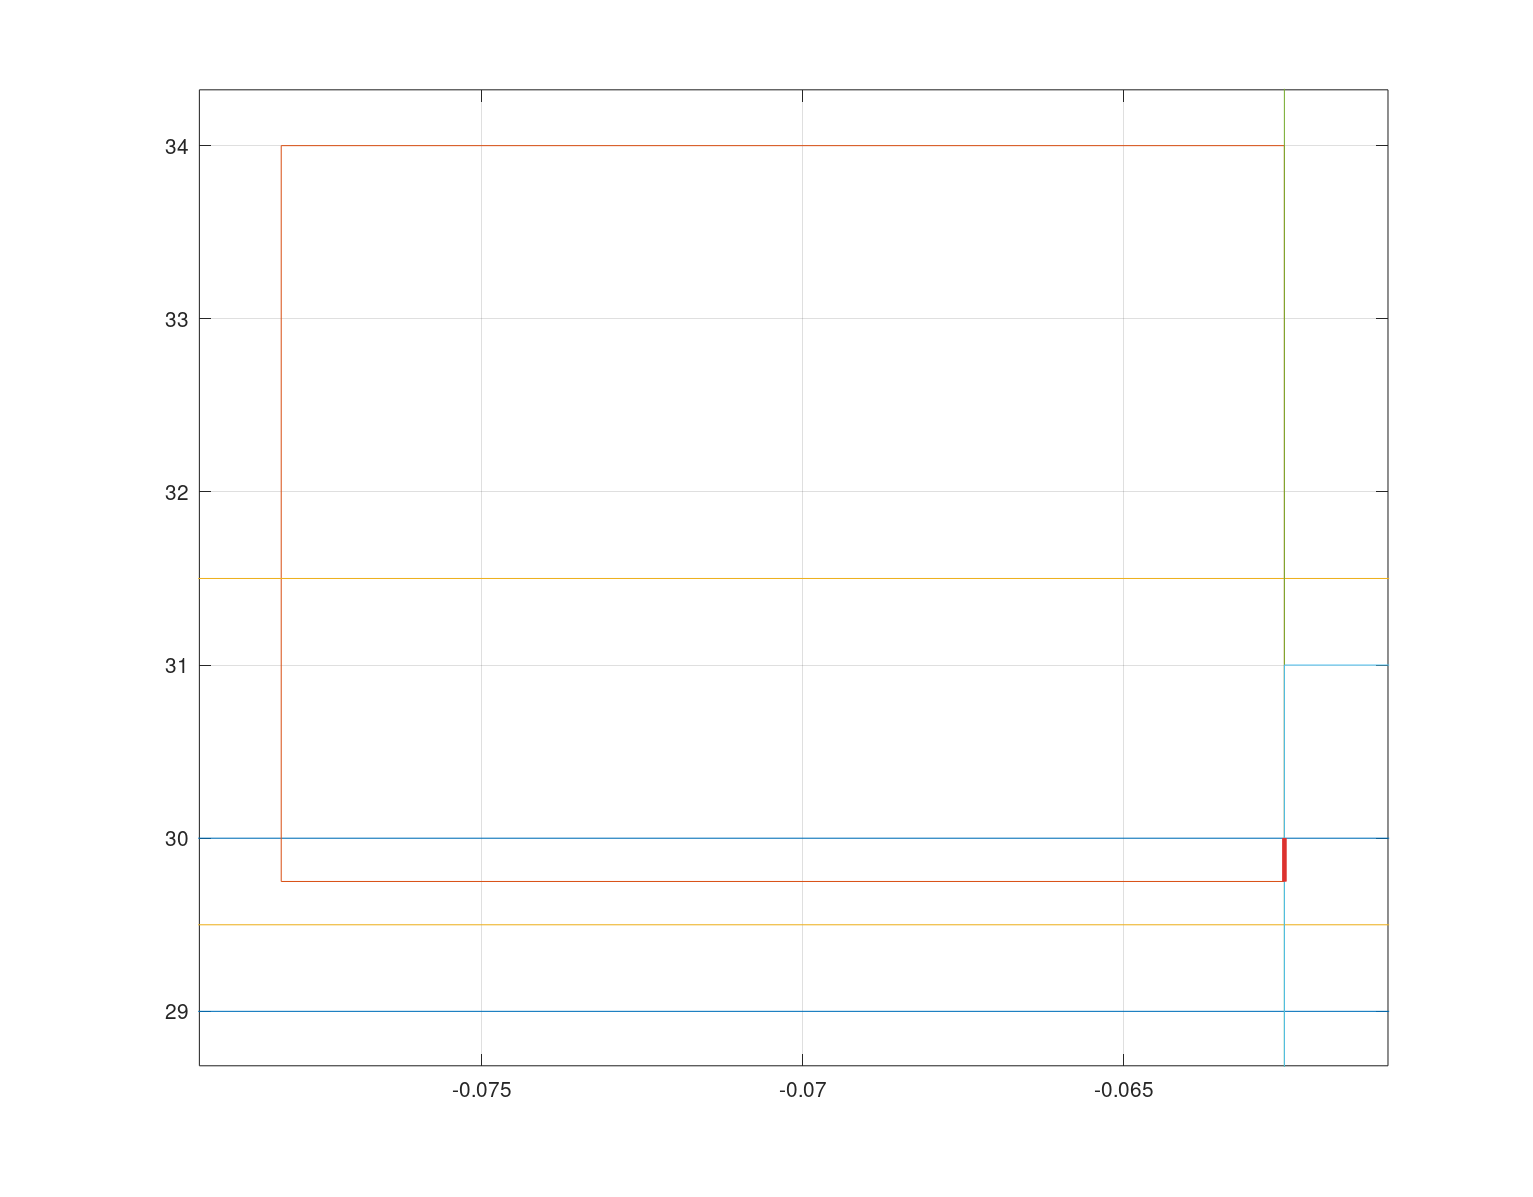
\includegraphics[width=8cm]{img/boxes_close.png}
    \caption{Брусы $\Xi_i$, полученные методом квадратных подсистем и множество $\Xi$}
    \label{fig:boxes}
\end{figure}
Численные результаты: $\Xi\approx\left(\begin{smallmatrix}[-0.0625,-0.0625]\\ [29.75,30]\end{smallmatrix}\right)$. Ввиду узости полученной оценки информационного множества был выбран только один набор параметров регрессии $\beta=\imid\Xi=\left(\begin{smallmatrix}-0.0625\\ 29.875\end{smallmatrix}\right)$. На следующем графике изображены исходные точечные данные, брусья, полученные после операции взятия минимумов по включению и полученная регрессионная прямая.
\begin{figure}[H]
    \centering
    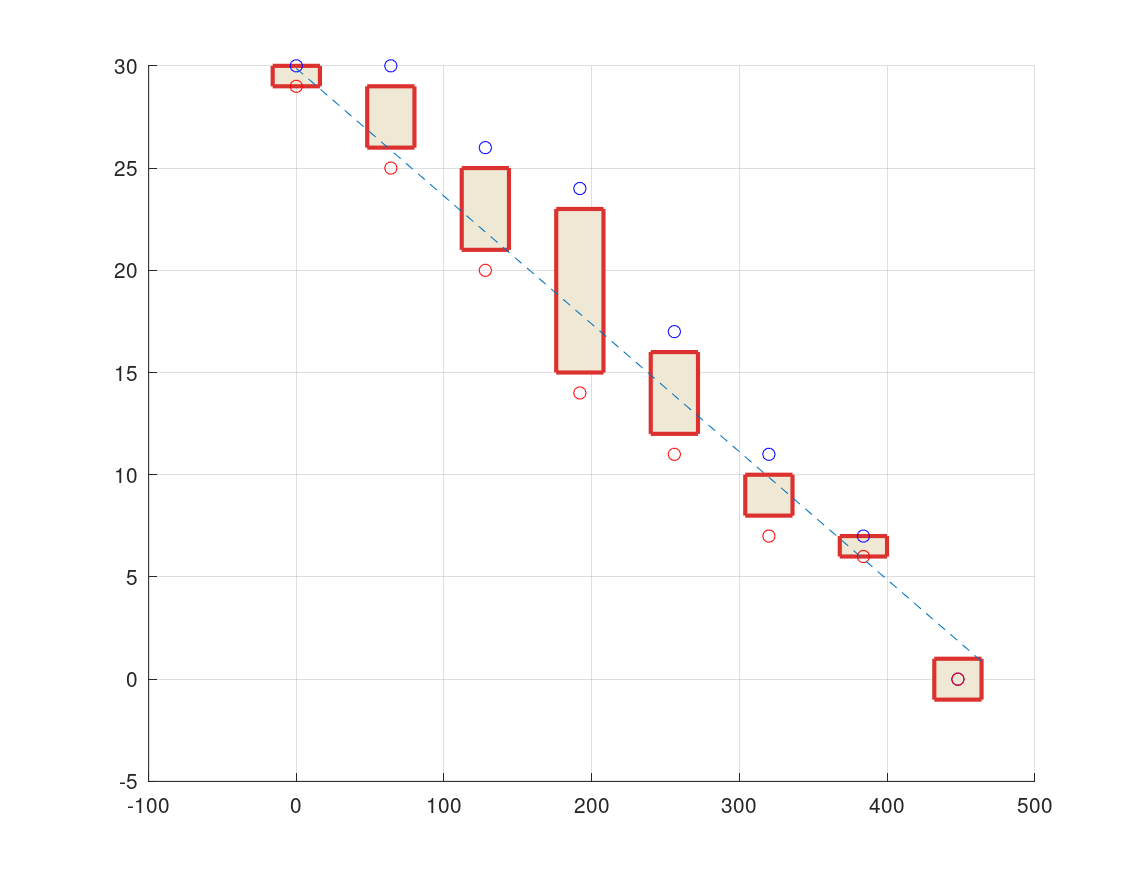
\includegraphics[width=15cm]{img/res_3.png}
    \caption{Результат построений с помощью обработки данных в $\mbb{KR}$}
    \label{fig:res_3}
\end{figure}
\section{Обсуждение}
\begin{enumerate}
    \item Как уже было описано, исходя из данных на графике \ref{fig:data} можно сделать вывод о характере входных данных: в исходной выборке имеются две квазилинейные подвыборки, обе отрицательно коррелированы.
    \item При достижении совместности этих ветвей по отдельности были получены практически параллельные прямые, смещенные друг относительно друга. 
    \item По графику \ref{fig:branches} видно, что алгоритм \ref{alg1} достиг своей цели: обе прямые подходят через полученные интервалы, совместность обоих выборок была достигнута минимальным суммарным расширением отклика. Информационное множество в обоих случаях состоит из одной точки, так как в обоих ветвях видны по 2 точечных величины, следовательно, прямая, проходящая через них, задается единственным образом. 
    \item По графику \ref{fig:branches} и численным результатам соответствующей процедуры видно, что нижняя ветвь содержит меньше отклонений от линейной зависимости: для достижения совместности в ее отклики пришлось вносить меньшую неопределенность.
    \item Ситуация с рассмотрением выборки в целом (график \ref{fig:res_1}) аналогична: информационное множество точечное - есть два точечных отклика. Можно отметить, что расширение, которое пришлось внести, значительно больше, чем сумма расширений для двух ветвей по отдельности. 
    \item В нижнюю ветвь все так же было внесено меньше неопределенности, чем в верхнюю: красные интервалы на графике \ref{fig:res_1} заметно уже синих.
    \item По графику \ref{fig:res_2} видно, что полученная зависимость действительно является сильно совместной - алгоритм \ref{alg2} достиг нужного результата. 
    \item Сравнивая коэффициенты $\beta_0$, полученные после обработки выборки алгоритмами \ref{alg1} и \ref{alg2}, приходим к выводу, что полученная с помощью алгоритма \ref{alg1} регрессия весьма оптимальна: даже при внесении дополнительной неопределенности в исходные данные прямая не нуждается в большой коррекции для обеспечения сильной совместности. 
    \item В ходе применения алгоритма \ref{alg2} исходные брусья были в небольшой степени расширены по отклику. По предиктору расширение внесено не было.
    \item Полученное в ходе обработки выборки третьим способом информационное множество получилось очень узким, практически точечным по параметру $\beta_1$. Это может быть объяснено как не самым удачным выбором матриц в методе квадратных подсистем (на графике \ref{fig:boxes} видно, что один из брусьев почти что вырождает пересечение по первой координате), так и не лучшей совместностью исходных данных.
    \item По графику \ref{fig:res_3} можно сделать вывод, что полученная регрессия обладает слабой совместностью с брусьями $\mbf{y}_k^1\bigwedge\mbf{y}_k^2$.
    \item Полученные тремя подходами результаты схожи: различие по параметру $\beta_1$ составляет около 7\%, по параметру $\beta_0$ - не более 2\%.
\end{enumerate}
\section*{Исходный код}
С исходным кодом программы и отчета можно ознакомиться в репозитории \url{https://github.com/Stasychbr/IntervalArith}.
\newpage
\begin{thebibliography}{9}
\bibitem[1]{book1} 
 А. Н. Баженов. Лекции по интервальному анализу. СПбПУ. 2021
 \url{https://cloud.mail.ru/public/VSFh/gJgtFVynE}
\bibitem[2]{book2} А. Н. Баженов. Интервальный анализ. Основы теории и учебные примеры: учебное пособие. - СПб. 2020 - 78 с.
\bibitem[3]{book3} С. И. Жилин. Библиотека kinterval. Код в Octave. Альфа версия. 2020.
\end{thebibliography}
\end{document}
